\documentclass[lettersize,journal]{IEEEtran}
\usepackage{amsmath,amsfonts}
\usepackage{algorithmic}
\usepackage{algorithm}
\usepackage{array}
\usepackage[caption=false,font=normalsize,labelfont=sf,textfont=sf]{subfig}
\usepackage{textcomp}
\usepackage{stfloats}
\usepackage{url}
\usepackage{verbatim}
\usepackage{graphicx}
\usepackage{cite}
\hyphenation{op-tical net-works semi-conduc-tor IEEE-Xplore}
% updated with editorial comments 8/9/2021

\begin{document}

\title{A Sample Article Using IEEEtran.cls\\ for IEEE Journals and Transactions}

\author{IEEE Publication Technology,~\IEEEmembership{Staff,~IEEE,}
        % <-this % stops a space
\thanks{This paper was produced by the IEEE Publication Technology Group. They are in Piscataway, NJ.}% <-this % stops a space
\thanks{Manuscript received April 19, 2021; revised August 16, 2021.}}

% The paper headers
\markboth{Journal of \LaTeX\ Class Files,~Vol.~14, No.~8, August~2021}%
{Shell \MakeLowercase{\textit{et al.}}: A Sample Article Using IEEEtran.cls for IEEE Journals}

\IEEEpubid{0000--0000/00\$00.00~\copyright~2021 IEEE}
% Remember, if you use this you must call \IEEEpubidadjcol in the second
% column for its text to clear the IEEEpubid mark.

\maketitle

\begin{abstract}
This document describes the most common article elements and how to use the IEEEtran class with \LaTeX \ to produce files that are suitable for submission to the IEEE.  IEEEtran can produce conference, journal, and technical note (correspondence) papers with a suitable choice of class options. 
\end{abstract}

\begin{IEEEkeywords}
Article submission, IEEE, IEEEtran, journal, \LaTeX, paper, template, typesetting.
\end{IEEEkeywords}

\section{Introduction}
\IEEEPARstart{W}{ith} climate change, renewable energy has become a crucial part of the energy transition in countries around the world, and the penetration rate of wind power has continued to rise accordingly. However, the randomness and intermittency of wind speeds, as well as forecasting errors, cause frequent fluctuations in the grid-connected power of wind farms~\cite{ref1}, which in turn affect power quality, dispatch reliability, and grid security~\cite{ref2,ref3}. Regarding power fluctuations caused by wind power, existing control methods fall into two main categories: one involves power smoothing solely by adjusting the wind turbine's pitch angle or axial induction factor. This method often results in a loss of wind energy utilization rate~\cite{ref4} and increases fatigue on the mechanical components of wind turbines~\cite{ref5}. The other category involves introducing energy storage facilities to form a Wind-Storage Integrated System (WSIS) in conjunction with the wind farm. By leveraging the power regulation capabilities of wind turbines and the rapid charging and discharging capabilities of energy storage, WSIS suppresses grid-connected power fluctuations while increasing power generation revenue, and has become a key solution for integrating high proportions of wind power into the grid~\cite{ref6}.

WSIS control requires coordinating wind turbines and energy storage systems with different dynamic characteristics and control frequencies: to avoid wind energy losses and mechanical fatigue caused by frequent adjustments to the wind turbines, the turbines typically optimize their overall power output on a slower time scale; meanwhile, the energy storage system tracks a smooth target on a faster time scale to achieve a smooth overall output~\cite{ref7}. Mainstream wind turbine control methods each have their own limitations and shortcomings: PID control relies on linearized model parameters; in wind power environments characterized by strong nonlinearity, high inertia, and time delays, it suffers from poor robustness, and parameter tuning is time-consuming and difficult; Model predictive control and rule-based control rely on accurate wake models~\cite{ref8}, wind speed forecasts, and battery models; in large-scale, highly uncertain environments, they suffer from complex modeling, high computational overhead~\cite{ref9,ref10}, and limited generalization ability~\cite{ref11}. Furthermore, there is a clear conflict between maximizing economic benefits and power fluctuation constraints~\cite{ref12}, which may result in overly conservative strategies or frequent violations of safety constraints.

To address the above issues, reinforcement learning (RL)---as a model-free approach that directly learns control policies through interaction with the environment without the need for prior modeling of system dynamics---offers a new approach to controlling complex WSIS systems~\cite{ref7,ref13}. Hierarchical Safe Reinforcement Learning (HSRL) utilizes different control time scales to decompose upper-level wind turbine scheduling and lower-level energy storage smoothing into mutually cooperative decision-making processes, while ensuring compliance with control constraints and objectives~\cite{ref14}. However, existing methods still face challenges such as reward boundaries relying on manual experience, difficulty in adapting boundaries to changing operating conditions, and training oscillations caused by inter-layer coupling and sample imbalance in constraints. To this end, this paper proposes an LLM-guided segmented reward reinforcement learning framework based on the HSRL framework~\cite{ref14}. By explicitly delineating different risk and profit zones through segment-based rewards, this approach utilizes a large language model (LLM) in conjunction with operational data to dynamically adjust segment boundaries, and employs a hierarchical dual-timescale objective network and a delayed strategy update to enhance training stability~\cite{ref15,ref16}.

A fixed penalty coefficient or a single continuous reward makes it difficult to simultaneously distinguish between the safe zone, the balanced zone, and the dangerous zone~\cite{ref17}, which may result in the policy becoming overly conservative or frequently violating safety constraints. Segmented Reward Function Reinforcement Learning (PRRL) offers a highly promising solution to this problem. This method employs different reward function formulas based on control objectives in various environments; for example, it emphasizes utility in the safe zone, balances utility and constraints in the balanced zone, and guides rapid stabilization while adhering to fluctuation constraints in the hazardous zone. Experiments have demonstrated that in air combat decision-making~\cite{ref18} and mobile robot navigation and close-following scenarios~\cite{ref19}, segmented reward models can significantly improve accuracy and stability in complex scenarios compared to single-value baseline reward models. On the other hand, Large Language Model-Enhanced Reinforcement Learning (LERL) provides a more efficient segmentation method for reinforcement learning agents using segmented reward functions. During training with segmented reward functions, precisely identifying the most appropriate segmentation boundaries is challenging due to the continuous nature of wind speeds in the WSIS environment. By using an LLM to fine-tune the segmentation boundaries based on data collected during training, an optimal partition can be obtained that balances constraint satisfaction with profit maximization. LLMs have been widely applied in various aspects of reinforcement learning~\cite{ref20}, such as serving as information processors to reduce learning complexity~\cite{ref21}, as reward designers to design reward functions in complex task environments~\cite{ref22}, and as decision-makers to generate or guide reliable actions to accelerate offline reinforcement learning~\cite{ref23}.

Although there has been extensive research in the academic community on both piecewise reward function reinforcement learning (PRRL) and LLM-enhanced RL (LERL), few studies have attempted to integrate PRRL and LERL to construct an LLM-enhanced piecewise reward function reinforcement learning (LEPRRL) framework. This integration presents several challenges, notably: 1) segmented reward functions introduce non-smooth reward surfaces at the boundaries, leading to high-variance gradient updates and cumulative overestimation; 2) fine-tuning of segmented boundaries by the LLM causes local shifts in the reward surface, resulting in Q-value estimates lagging behind surface changes and affecting the accuracy of policy updates. To address these limitations, this paper proposes an LLM-enhanced segmented reward reinforcement learning (LEPRRL) framework based on the TD3 algorithm for the WSIS control problem, building upon the HSRL framework~\cite{ref14}. Its contributions are as follows:

\begin{enumerate}
\item A piecewise reward function method is proposed. By guiding the agent to pursue different objectives in different segments, this method improves control performance and operational safety, thereby resolving the challenge of balancing reward optimization with safety constraints.

\item A method for LLM-enhanced reinforcement learning is proposed. By utilizing an LLM to monitor parameters and fine-tune segmentation logic during training, this method identifies optimal segmentation points and optimizes the agent's overall performance.

\item To address the training instability introduced by the aforementioned segmented reward mechanism and LLM boundary fine-tuning, we introduce a TD3-based dual-Q-network and delayed policy update framework, which ensures the convergence stability of the LEPRRL framework during long-time-domain training.
\end{enumerate}

\section{The Design, Intent, and \\ Limitations of the Templates}
The templates are intended to {\bf{approximate the final look and page length of the articles/papers}}. {\bf{They are NOT intended to be the final produced work that is displayed in print or on IEEEXplore\textsuperscript{\textregistered}}}. They will help to give the authors an approximation of the number of pages that will be in the final version. The structure of the \LaTeX\ files, as designed, enable easy conversion to XML for the composition systems used by the IEEE. The XML files are used to produce the final print/IEEEXplore pdf and then converted to HTML for IEEEXplore.

\section{Where to Get \LaTeX \ Help --- User Groups}
The following online groups are helpful to beginning and experienced \LaTeX\ users. A search through their archives can provide many answers to common questions.
\begin{list}{}{}
\item{\url{http://www.latex-community.org/}} 
\item{\url{https://tex.stackexchange.com/} }
\end{list}

\section{Other Resources}
See \cite{ref1,ref2,ref3,ref4,ref5} for resources on formatting math into text and additional help in working with \LaTeX .

\section{Text}
For some of the remainer of this sample we will use dummy text to fill out paragraphs rather than use live text that may violate a copyright.

Itam, que ipiti sum dem velit la sum et dionet quatibus apitet voloritet audam, qui aliciant voloreicid quaspe volorem ut maximusandit faccum conemporerum aut ellatur, nobis arcimus.
Fugit odi ut pliquia incitium latum que cusapere perit molupta eaquaeria quod ut optatem poreiur? Quiaerr ovitior suntiant litio bearciur?

Onseque sequaes rectur autate minullore nusae nestiberum, sum voluptatio. Et ratem sequiam quaspername nos rem repudandae volum consequis nos eium aut as molupta tectum ulparumquam ut maximillesti consequas quas inctia cum volectinusa porrum unt eius cusaest exeritatur? Nias es enist fugit pa vollum reium essusam nist et pa aceaqui quo elibusdandis deligendus que nullaci lloreri bla que sa coreriam explacc atiumquos simolorpore, non prehendunt lam que occum\cite{ref6} si aut aut maximus eliaeruntia dia sequiamenime natem sendae ipidemp orehend uciisi omnienetus most verum, ommolendi omnimus, est, veni aut ipsa volendelist mo conserum volores estisciis recessi nveles ut poressitatur sitiis ex endi diti volum dolupta aut aut odi as eatquo cullabo remquis toreptum et des accus dolende pores sequas dolores tinust quas expel moditae ne sum quiatis nis endipie nihilis etum fugiae audi dia quiasit quibus.
\IEEEpubidadjcol
Ibus el et quatemo luptatque doluptaest et pe volent rem ipidusa eribus utem venimolorae dera qui acea quam etur aceruptat.
Gias anis doluptaspic tem et aliquis alique inctiuntiur?

Sedigent, si aligend elibuscid ut et ium volo tem eictore pellore ritatus ut ut ullatus in con con pere nos ab ium di tem aliqui od magnit repta volectur suntio. Nam isquiante doluptis essit, ut eos suntionsecto debitiur sum ea ipitiis adipit, oditiore, a dolorerempos aut harum ius, atquat.

Rum rem ditinti sciendunti volupiciendi sequiae nonsect oreniatur, volores sition ressimil inus solut ea volum harumqui to see\eqref{deqn_ex1a} mint aut quat eos explis ad quodi debis deliqui aspel earcius.

\begin{equation}
\label{deqn_ex1a}
x = \sum_{i=0}^{n} 2{i} Q.
\end{equation}

Alis nime volorempera perferi sitio denim repudae pre ducilit atatet volecte ssimillorae dolore, ut pel ipsa nonsequiam in re nus maiost et que dolor sunt eturita tibusanis eatent a aut et dio blaudit reptibu scipitem liquia consequodi od unto ipsae. Et enitia vel et experferum quiat harum sa net faccae dolut voloria nem. Bus ut labo. Ita eum repraer rovitia samendit aut et volupta tecupti busant omni quiae porro que nossimodic temquis anto blacita conse nis am, que ereperum eumquam quaescil imenisci quae magnimos recus ilibeaque cum etum iliate prae parumquatemo blaceaquiam quundia dit apienditem rerit re eici quaes eos sinvers pelecabo. Namendignis as exerupit aut magnim ium illabor roratecte plic tem res apiscipsam et vernat untur a deliquaest que non cus eat ea dolupiducim fugiam volum hil ius dolo eaquis sitis aut landesto quo corerest et auditaquas ditae voloribus, qui optaspis exero cusa am, ut plibus.


\section{Some Common Elements}
\subsection{Sections and Subsections}
Enumeration of section headings is desirable, but not required. When numbered, please be consistent throughout the article, that is, all headings and all levels of section headings in the article should be enumerated. Primary headings are designated with Roman numerals, secondary with capital letters, tertiary with Arabic numbers; and quaternary with lowercase letters. Reference and Acknowledgment headings are unlike all other section headings in text. They are never enumerated. They are simply primary headings without labels, regardless of whether the other headings in the article are enumerated. 

\subsection{Citations to the Bibliography}
The coding for the citations is made with the \LaTeX\ $\backslash${\tt{cite}} command. 
This will display as: see \cite{ref1}.

For multiple citations code as follows: {\tt{$\backslash$cite\{ref1,ref2,ref3\}}}
 which will produce \cite{ref1,ref2,ref3}. For reference ranges that are not consecutive code as {\tt{$\backslash$cite\{ref1,ref2,ref3,ref9\}}} which will produce  \cite{ref1,ref2,ref3,ref9}

\subsection{Lists}
In this section, we will consider three types of lists: simple unnumbered, numbered, and bulleted. There have been many options added to IEEEtran to enhance the creation of lists. If your lists are more complex than those shown below, please refer to the original ``IEEEtran\_HOWTO.pdf'' for additional options.\\

\subsubsection*{\bf A plain  unnumbered list}
\begin{list}{}{}
\item{bare\_jrnl.tex}
\item{bare\_conf.tex}
\item{bare\_jrnl\_compsoc.tex}
\item{bare\_conf\_compsoc.tex}
\item{bare\_jrnl\_comsoc.tex}
\end{list}

\subsubsection*{\bf A simple numbered list}
\begin{enumerate}
\item{bare\_jrnl.tex}
\item{bare\_conf.tex}
\item{bare\_jrnl\_compsoc.tex}
\item{bare\_conf\_compsoc.tex}
\item{bare\_jrnl\_comsoc.tex}
\end{enumerate}

\subsubsection*{\bf A simple bulleted list}
\begin{itemize}
\item{bare\_jrnl.tex}
\item{bare\_conf.tex}
\item{bare\_jrnl\_compsoc.tex}
\item{bare\_conf\_compsoc.tex}
\item{bare\_jrnl\_comsoc.tex}
\end{itemize}





\subsection{Figures}
Fig. 1 is an example of a floating figure using the graphicx package.
 Note that $\backslash${\tt{label}} must occur AFTER (or within) $\backslash${\tt{caption}}.
 For figures, $\backslash${\tt{caption}} should occur after the $\backslash${\tt{includegraphics}}.

\begin{figure}[!t]
\centering
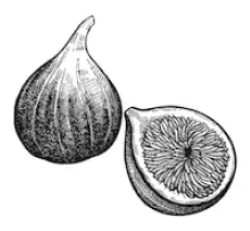
\includegraphics[width=2.5in]{fig1}
\caption{Simulation results for the network.}
\label{fig_1}
\end{figure}

Fig. 2(a) and 2(b) is an example of a double column floating figure using two subfigures.
 (The subfig.sty package must be loaded for this to work.)
 The subfigure $\backslash${\tt{label}} commands are set within each subfloat command,
 and the $\backslash${\tt{label}} for the overall figure must come after $\backslash${\tt{caption}}.
 $\backslash${\tt{hfil}} is used as a separator to get equal spacing.
 The combined width of all the parts of the figure should do not exceed the text width or a line break will occur.
%
\begin{figure*}[!t]
\centering
\subfloat[]{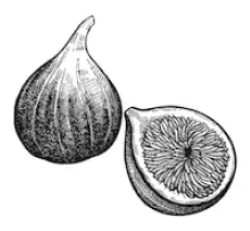
\includegraphics[width=2.5in]{fig1}%
\label{fig_first_case}}
\hfil
\subfloat[]{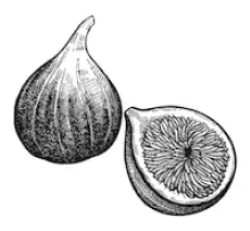
\includegraphics[width=2.5in]{fig1}%
\label{fig_second_case}}
\caption{Dae. Ad quatur autat ut porepel itemoles dolor autem fuga. Bus quia con nessunti as remo di quatus non perum que nimus. (a) Case I. (b) Case II.}
\label{fig_sim}
\end{figure*}

Note that often IEEE papers with multi-part figures do not place the labels within the image itself (using the optional argument to $\backslash${\tt{subfloat}}[]), but instead will
 reference/describe all of them (a), (b), etc., within the main caption.
 Be aware that for subfig.sty to generate the (a), (b), etc., subfigure
 labels, the optional argument to $\backslash${\tt{subfloat}} must be present. If a
 subcaption is not desired, leave its contents blank,
 e.g.,$\backslash${\tt{subfloat}}[].


 

\section{Tables}
Note that, for IEEE-style tables, the
 $\backslash${\tt{caption}} command should come BEFORE the table. Table captions use title case. Articles (a, an, the), coordinating conjunctions (and, but, for, or, nor), and most short prepositions are lowercase unless they are the first or last word. Table text will default to $\backslash${\tt{footnotesize}} as
 the IEEE normally uses this smaller font for tables.
 The $\backslash${\tt{label}} must come after $\backslash${\tt{caption}} as always.
 
\begin{table}[!t]
\caption{An Example of a Table\label{tab:table1}}
\centering
\begin{tabular}{|c||c|}
\hline
One & Two\\
\hline
Three & Four\\
\hline
\end{tabular}
\end{table}

\section{Algorithms}
Algorithms should be numbered and include a short title. They are set off from the text with rules above and below the title and after the last line.

\begin{algorithm}[H]
\caption{Weighted Tanimoto ELM.}\label{alg:alg1}
\begin{algorithmic}
\STATE 
\STATE {\textsc{TRAIN}}$(\mathbf{X} \mathbf{T})$
\STATE \hspace{0.5cm}$ \textbf{select randomly } W \subset \mathbf{X}  $
\STATE \hspace{0.5cm}$ N_\mathbf{t} \gets | \{ i : \mathbf{t}_i = \mathbf{t} \} | $ \textbf{ for } $ \mathbf{t}= -1,+1 $
\STATE \hspace{0.5cm}$ B_i \gets \sqrt{ \textsc{max}(N_{-1},N_{+1}) / N_{\mathbf{t}_i} } $ \textbf{ for } $ i = 1,...,N $
\STATE \hspace{0.5cm}$ \hat{\mathbf{H}} \gets  B \cdot (\mathbf{X}^T\textbf{W})/( \mathbb{1}\mathbf{X} + \mathbb{1}\textbf{W} - \mathbf{X}^T\textbf{W} ) $
\STATE \hspace{0.5cm}$ \beta \gets \left ( I/C + \hat{\mathbf{H}}^T\hat{\mathbf{H}} \right )^{-1}(\hat{\mathbf{H}}^T B\cdot \mathbf{T})  $
\STATE \hspace{0.5cm}\textbf{return}  $\textbf{W},  \beta $
\STATE 
\STATE {\textsc{PREDICT}}$(\mathbf{X} )$
\STATE \hspace{0.5cm}$ \mathbf{H} \gets  (\mathbf{X}^T\textbf{W} )/( \mathbb{1}\mathbf{X}  + \mathbb{1}\textbf{W}- \mathbf{X}^T\textbf{W}  ) $
\STATE \hspace{0.5cm}\textbf{return}  $\textsc{sign}( \mathbf{H} \beta )$
\end{algorithmic}
\label{alg1}
\end{algorithm}

Que sunt eum lam eos si dic to estist, culluptium quid qui nestrum nobis reiumquiatur minimus minctem. Ro moluptat fuga. Itatquiam ut laborpo rersped exceres vollandi repudaerem. Ulparci sunt, qui doluptaquis sumquia ndestiu sapient iorepella sunti veribus. Ro moluptat fuga. Itatquiam ut laborpo rersped exceres vollandi repudaerem. 
\section{Mathematical Typography \\ and Why It Matters}

Typographical conventions for mathematical formulas have been developed to {\bf provide uniformity and clarity of presentation across mathematical texts}. This enables the readers of those texts to both understand the author's ideas and to grasp new concepts quickly. While software such as \LaTeX \ and MathType\textsuperscript{\textregistered} can produce aesthetically pleasing math when used properly, it is also very easy to misuse the software, potentially resulting in incorrect math display.

IEEE aims to provide authors with the proper guidance on mathematical typesetting style and assist them in writing the best possible article. As such, IEEE has assembled a set of examples of good and bad mathematical typesetting \cite{ref1,ref2,ref3,ref4,ref5}. 

Further examples can be found at \url{http://journals.ieeeauthorcenter.ieee.org/wp-content/uploads/sites/7/IEEE-Math-Typesetting-Guide-for-LaTeX-Users.pdf}

\subsection{Display Equations}
The simple display equation example shown below uses the ``equation'' environment. To number the equations, use the $\backslash${\tt{label}} macro to create an identifier for the equation. LaTeX will automatically number the equation for you.
\begin{equation}
\label{deqn_ex1}
x = \sum_{i=0}^{n} 2{i} Q.
\end{equation}

\noindent is coded as follows:
\begin{verbatim}
\begin{equation}
\label{deqn_ex1}
x = \sum_{i=0}^{n} 2{i} Q.
\end{equation}
\end{verbatim}

To reference this equation in the text use the $\backslash${\tt{ref}} macro. 
Please see (\ref{deqn_ex1})\\
\noindent is coded as follows:
\begin{verbatim}
Please see (\ref{deqn_ex1})\end{verbatim}

\subsection{Equation Numbering}
{\bf{Consecutive Numbering:}} Equations within an article are numbered consecutively from the beginning of the
article to the end, i.e., (1), (2), (3), (4), (5), etc. Do not use roman numerals or section numbers for equation numbering.

\noindent {\bf{Appendix Equations:}} The continuation of consecutively numbered equations is best in the Appendix, but numbering
 as (A1), (A2), etc., is permissible.\\

\noindent {\bf{Hyphens and Periods}}: Hyphens and periods should not be used in equation numbers, i.e., use (1a) rather than
(1-a) and (2a) rather than (2.a) for subequations. This should be consistent throughout the article.

\subsection{Multi-Line Equations and Alignment}
Here we show several examples of multi-line equations and proper alignments.

\noindent {\bf{A single equation that must break over multiple lines due to length with no specific alignment.}}
\begin{multline}
\text{The first line of this example}\\
\text{The second line of this example}\\
\text{The third line of this example}
\end{multline}

\noindent is coded as:
\begin{verbatim}
\begin{multline}
\text{The first line of this example}\\
\text{The second line of this example}\\
\text{The third line of this example}
\end{multline}
\end{verbatim}

\noindent {\bf{A single equation with multiple lines aligned at the = signs}}
\begin{align}
a &= c+d \\
b &= e+f
\end{align}
\noindent is coded as:
\begin{verbatim}
\begin{align}
a &= c+d \\
b &= e+f
\end{align}
\end{verbatim}

The {\tt{align}} environment can align on multiple  points as shown in the following example:
\begin{align}
x &= y & X & =Y & a &=bc\\
x' &= y' & X' &=Y' &a' &=bz
\end{align}
\noindent is coded as:
\begin{verbatim}
\begin{align}
x &= y & X & =Y & a &=bc\\
x' &= y' & X' &=Y' &a' &=bz
\end{align}
\end{verbatim}





\subsection{Subnumbering}
The amsmath package provides a {\tt{subequations}} environment to facilitate subnumbering. An example:

\begin{subequations}\label{eq:2}
\begin{align}
f&=g \label{eq:2A}\\
f' &=g' \label{eq:2B}\\
\mathcal{L}f &= \mathcal{L}g \label{eq:2c}
\end{align}
\end{subequations}

\noindent is coded as:
\begin{verbatim}
\begin{subequations}\label{eq:2}
\begin{align}
f&=g \label{eq:2A}\\
f' &=g' \label{eq:2B}\\
\mathcal{L}f &= \mathcal{L}g \label{eq:2c}
\end{align}
\end{subequations}

\end{verbatim}

\subsection{Matrices}
There are several useful matrix environments that can save you some keystrokes. See the example coding below and the output.

\noindent {\bf{A simple matrix:}}
\begin{equation}
\begin{matrix}  0 &  1 \\ 
1 &  0 \end{matrix}
\end{equation}
is coded as:
\begin{verbatim}
\begin{equation}
\begin{matrix}  0 &  1 \\ 
1 &  0 \end{matrix}
\end{equation}
\end{verbatim}

\noindent {\bf{A matrix with parenthesis}}
\begin{equation}
\begin{pmatrix} 0 & -i \\
 i &  0 \end{pmatrix}
\end{equation}
is coded as:
\begin{verbatim}
\begin{equation}
\begin{pmatrix} 0 & -i \\
 i &  0 \end{pmatrix}
\end{equation}
\end{verbatim}

\noindent {\bf{A matrix with square brackets}}
\begin{equation}
\begin{bmatrix} 0 & -1 \\ 
1 &  0 \end{bmatrix}
\end{equation}
is coded as:
\begin{verbatim}
\begin{equation}
\begin{bmatrix} 0 & -1 \\ 
1 &  0 \end{bmatrix}
\end{equation}
\end{verbatim}

\noindent {\bf{A matrix with curly braces}}
\begin{equation}
\begin{Bmatrix} 1 &  0 \\ 
0 & -1 \end{Bmatrix}
\end{equation}
is coded as:
\begin{verbatim}
\begin{equation}
\begin{Bmatrix} 1 &  0 \\ 
0 & -1 \end{Bmatrix}
\end{equation}\end{verbatim}

\noindent {\bf{A matrix with single verticals}}
\begin{equation}
\begin{vmatrix} a &  b \\ 
c &  d \end{vmatrix}
\end{equation}
is coded as:
\begin{verbatim}
\begin{equation}
\begin{vmatrix} a &  b \\ 
c &  d \end{vmatrix}
\end{equation}\end{verbatim}

\noindent {\bf{A matrix with double verticals}}
\begin{equation}
\begin{Vmatrix} i &  0 \\ 
0 & -i \end{Vmatrix}
\end{equation}
is coded as:
\begin{verbatim}
\begin{equation}
\begin{Vmatrix} i &  0 \\ 
0 & -i \end{Vmatrix}
\end{equation}\end{verbatim}

\subsection{Arrays}
The {\tt{array}} environment allows you some options for matrix-like equations. You will have to manually key the fences, but there are other options for alignment of the columns and for setting horizontal and vertical rules. The argument to {\tt{array}} controls alignment and placement of vertical rules.

A simple array
\begin{equation}
\left(
\begin{array}{cccc}
a+b+c & uv & x-y & 27\\
a+b & u+v & z & 134
\end{array}\right)
\end{equation}
is coded as:
\begin{verbatim}
\begin{equation}
\left(
\begin{array}{cccc}
a+b+c & uv & x-y & 27\\
a+b & u+v & z & 134
\end{array} \right)
\end{equation}
\end{verbatim}

A slight variation on this to better align the numbers in the last column
\begin{equation}
\left(
\begin{array}{cccr}
a+b+c & uv & x-y & 27\\
a+b & u+v & z & 134
\end{array}\right)
\end{equation}
is coded as:
\begin{verbatim}
\begin{equation}
\left(
\begin{array}{cccr}
a+b+c & uv & x-y & 27\\
a+b & u+v & z & 134
\end{array} \right)
\end{equation}
\end{verbatim}

An array with vertical and horizontal rules
\begin{equation}
\left( \begin{array}{c|c|c|r}
a+b+c & uv & x-y & 27\\ \hline
a+b & u+v & z & 134
\end{array}\right)
\end{equation}
is coded as:
\begin{verbatim}
\begin{equation}
\left(
\begin{array}{c|c|c|r}
a+b+c & uv & x-y & 27\\
a+b & u+v & z & 134
\end{array} \right)
\end{equation}
\end{verbatim}
Note the argument now has the pipe "$\vert$" included to indicate the placement of the vertical rules.


\subsection{Cases Structures}
Many times cases can be miscoded using the wrong environment, i.e., {\tt{array}}. Using the {\tt{cases}} environment will save keystrokes (from not having to type the $\backslash${\tt{left}}$\backslash${\tt{lbrace}}) and automatically provide the correct column alignment.
\begin{equation*}
{z_m(t)} = \begin{cases}
1,&{\text{if}}\ {\beta }_m(t) \\ 
{0,}&{\text{otherwise.}} 
\end{cases}
\end{equation*}
\noindent is coded as follows:
\begin{verbatim}
\begin{equation*}
{z_m(t)} = 
\begin{cases}
1,&{\text{if}}\ {\beta }_m(t),\\ 
{0,}&{\text{otherwise.}} 
\end{cases}
\end{equation*}
\end{verbatim}
\noindent Note that the ``\&'' is used to mark the tabular alignment. This is important to get  proper column alignment. Do not use $\backslash${\tt{quad}} or other fixed spaces to try and align the columns. Also, note the use of the $\backslash${\tt{text}} macro for text elements such as ``if'' and ``otherwise.''

\subsection{Function Formatting in Equations}
Often, there is an easy way to properly format most common functions. Use of the $\backslash$ in front of the function name will in most cases, provide the correct formatting. When this does not work, the following example provides a solution using the $\backslash${\tt{text}} macro:

\begin{equation*} 
  d_{R}^{KM} = \underset {d_{l}^{KM}} {\text{arg min}} \{ d_{1}^{KM},\ldots,d_{6}^{KM}\}.
\end{equation*}

\noindent is coded as follows:
\begin{verbatim}
\begin{equation*} 
 d_{R}^{KM} = \underset {d_{l}^{KM}} 
 {\text{arg min}} \{ d_{1}^{KM},
 \ldots,d_{6}^{KM}\}.
\end{equation*}
\end{verbatim}

\subsection{ Text Acronyms Inside Equations}
This example shows where the acronym ``MSE" is coded using $\backslash${\tt{text\{\}}} to match how it appears in the text.

\begin{equation*}
 \text{MSE} = \frac {1}{n}\sum _{i=1}^{n}(Y_{i} - \hat {Y_{i}})^{2}
\end{equation*}

\begin{verbatim}
\begin{equation*}
 \text{MSE} = \frac {1}{n}\sum _{i=1}^{n}
(Y_{i} - \hat {Y_{i}})^{2}
\end{equation*}
\end{verbatim}

\section{Conclusion}
The conclusion goes here.


\section*{Acknowledgments}
This should be a simple paragraph before the References to thank those individuals and institutions who have supported your work on this article.



{\appendix[Proof of the Zonklar Equations]
Use $\backslash${\tt{appendix}} if you have a single appendix:
Do not use $\backslash${\tt{section}} anymore after $\backslash${\tt{appendix}}, only $\backslash${\tt{section*}}.
If you have multiple appendixes use $\backslash${\tt{appendices}} then use $\backslash${\tt{section}} to start each appendix.
You must declare a $\backslash${\tt{section}} before using any $\backslash${\tt{subsection}} or using $\backslash${\tt{label}} ($\backslash${\tt{appendices}} by itself
 starts a section numbered zero.)}



%{\appendices
%\section*{Proof of the First Zonklar Equation}
%Appendix one text goes here.
% You can choose not to have a title for an appendix if you want by leaving the argument blank
%\section*{Proof of the Second Zonklar Equation}
%Appendix two text goes here.}



\section{References Section}
You can use a bibliography generated by BibTeX as a .bbl file.
 BibTeX documentation can be easily obtained at:
 http://mirror.ctan.org/biblio/bibtex/contrib/doc/
 The IEEEtran BibTeX style support page is:
 http://www.michaelshell.org/tex/ieeetran/bibtex/
 
 % argument is your BibTeX string definitions and bibliography database(s)
%\bibliography{IEEEabrv,../bib/paper}
%
\section{Simple References}
You can manually copy in the resultant .bbl file and set second argument of $\backslash${\tt{begin}} to the number of references
 (used to reserve space for the reference number labels box).

\begin{thebibliography}{23}
\bibliographystyle{IEEEtran}

% =====================================================================
% 参考文献（23 条，编号按 Introduction 中首次出现顺序排列）。
% 条目依据下载 PDF 原文（"阅读材料\自找的参考文献"）提取。
% 说明：
%  - 原草稿编号仅用于对应 PDF；此处已按正文出现顺序重编号。
%  - 13.1.pdf 与 [7] 为同一篇文献（EPSR 255 (2026) 112707），已合并，
%    正文 RL 句复引第 7 条；
%  - ref6 为《中国电力》中文论文，用英文译题并标注 (in Chinese)；
%  - ref21/ref23 为 arXiv 预印本；ref22 为 ICLR 会议论文；
%  - ref19/ref23 作者众多：ref19 全部列出，ref23 按 IEEE 惯例用
%    "M. Ahn et al."（46 位作者全文见 arXiv:2204.01691）。
% =====================================================================

% REF1 (源 [1]) 风速随机性/间歇性及预测误差导致风电场并网出力频繁波动
\bibitem{ref1}
A. Michiorri, J. Lugaro, N. Siebert, R. Girard, and G. Kariniotakis, ``Storage sizing for grid connected hybrid wind and storage power plants taking into account forecast errors autocorrelation,'' \textit{Renewable Energy}, vol. 117, pp. 380--392, 2018, doi: 10.1016/j.renene.2017.10.070.

% REF2 (源 [2]) 并网功率波动影响电能质量
\bibitem{ref2}
E. Rahimi, A. Rabiee, J. Aghaei, K. M. Muttaqi, and A. Esmaeel Nezhad, ``On the management of wind power intermittency,'' \textit{Renewable and Sustainable Energy Reviews}, vol. 28, pp. 643--653, 2013, doi: 10.1016/j.rser.2013.08.034.

% REF3 (源 [3]) 风电大规模并网影响调度可靠性与电网安全
\bibitem{ref3}
T. Nam, J. W. Shim, and K. Hur, ``The beneficial role of SMES coil in DC lines as an energy buffer for integrating large scale wind power,'' \textit{IEEE Trans. Appl. Supercond.}, vol. 22, no. 3, Jun. 2012, Art. no. 5701404, doi: 10.1109/TASC.2011.2175686.

% REF4 (源 [4]) 仅靠变桨调节平滑功率会损失风能利用效率（会议论文，PDF 未印页码）
\bibitem{ref4}
Y. Li and Z. Xu, ``Power smoothing control of wind turbines using different strategies,'' in \textit{Proc. IEEE Int. Conf. Smart Grid Commun. (SmartGridComm)}, Sydney, Australia, 2016, doi: 10.1109/SmartGridComm.2016.7778844.

% REF5 (源 [5]) 频繁桨距角操纵导致桨距伺服系统明显疲劳
\bibitem{ref5}
X. Tang, M. Yin, C. Shen, Y. Xu, Z. Y. Dong, and Y. Zou, ``Active power control of wind turbine generators via coordinated rotor speed and pitch angle regulation,'' \textit{IEEE Trans. Sustain. Energy}, vol. 10, no. 2, pp. 822--832, Apr. 2019, doi: 10.1109/TSTE.2018.2848923.

% REF6 (源 [6]) WSIS 应用实例；原题（中文）：分散式风储一体化系统提升海上油田群电网频率稳定性研究（《中国电力》）
\bibitem{ref6}
K. Su, W. Dong, Y. Qiu, C. Wei, and X. Xie, ``Study on using distributed wind-storage integrated system to improve frequency stability of offshore oilfield power systems,'' \textit{Electric Power}, vol. 56, no. 5, pp. 163--171, 2023 (in Chinese), doi: 10.11930/j.issn.1004-9649.202205103.

% REF7 (源 [7]=13.1) 风机与储能不同时间尺度协调；RL 无模型控制 WSIS（正文两处引用）
\bibitem{ref7}
S. Wang, J. Zhao, H. Zhao, Y. Cao, Z. Pan, G. Liu, and G. Liang, ``Coordinated power smoothing control for wind storage integrated system with physics-informed deep reinforcement learning,'' \textit{Electric Power Systems Research}, vol. 255, Art. no. 112707, 2026, doi: 10.1016/j.epsr.2025.112707.

% REF8 (源 [8]) MPC/基于模型的控制依赖准确的尾流（延迟）模型（正式期次 2026-01，©2025）
\bibitem{ref8}
Y. Liu, J. Lin, L.-l. Huang, C. Hua, R. Huang, and Y. Fu, ``LPV model predictive control for offshore wind farms considering wake delay characteristics,'' \textit{IEEE Trans. Sustain. Energy}, vol. 17, no. 1, pp. 217--229, Jan. 2026, doi: 10.1109/TSTE.2025.3589608.

% REF9 (源 [9]) 高保真风电建模/预测计算开销大（尾流模型计算成本）
\bibitem{ref9}
Z. Ti, X. W. Deng, and M. Zhang, ``Artificial neural networks based wake model for power prediction of wind farm,'' \textit{Renewable Energy}, vol. 172, pp. 618--631, 2021, doi: 10.1016/j.renene.2021.03.030.

% REF10 (源 [10]) 风电功率预测模型计算开销大（轻量化需求）
\bibitem{ref10}
Y. Jin, M. Liu, Z. Lai, X. Cheng, and X. Liu, ``LightWind: A lightweight framework for efficient wind power forecasting,'' \textit{IEEE Sensors J.}, vol. 25, no. 19, pp. 36691--36703, Oct. 2025, doi: 10.1109/JSEN.2025.3600483.

% REF11 (源 [11]) 深度/机器学习模型在新场景下泛化能力弱
\bibitem{ref11}
H. Jin, G. Yang, S. Dong, S. Fan, H. Jin, and B. Wang, ``Wind power forecasting for newly built wind farms based on deep learning with dual-stage attention mechanism and adaptive transfer learning,'' \textit{Energy}, vol. 335, Art. no. 138275, 2025, doi: 10.1016/j.energy.2025.138275.

% REF12 (源 [12]) 最大化经济收益与（电网/多目标）约束之间的控制冲突
\bibitem{ref12}
Y. Huang and X. Zhao, ``Reinforcement learning-based multiobjective control of grid-connected wind farms,'' \textit{IEEE Trans. Ind. Informat.}, vol. 20, no. 5, pp. 7380--7390, May 2024, doi: 10.1109/TII.2024.3359420.

% REF13 (源 13.2) RL（MATD3）无需尾流模型的风储协调有功控制——模型无关 RL 用于 WSIS
\bibitem{ref13}
Q. Yao, Z. Liang, Y. Guan, Y. Ke, Y. Hu, F. Fang, and J. Liu, ``Wake model-free active power control for wind-storage coordination using a state-decoupled MATD3 algorithm,'' \textit{Energy}, vol. 347, Art. no. 140265, 2026, doi: 10.1016/j.energy.2026.140265.

% REF14 (源 [14]) 分层强化学习用于风储一体化功率平滑（HSRL，上层调度/下层平抑）
\bibitem{ref14}
S. Wang, H. Zhao, T. Shu, Z. Pan, G. Liang, and J. Zhao, ``Power smoothing control for wind-storage integrated systems with hierarchical safe reinforcement learning and curriculum learning,'' \textit{IEEE Trans. Smart Grid}, vol. 16, no. 6, pp. 4606--4619, Nov. 2025, doi: 10.1109/TSG.2025.3593340.

% REF15 (源 [15]) TD3 原文：双 Critic + 延迟策略更新提升训练稳定性
\bibitem{ref15}
S. Fujimoto, H. van Hoof, and D. Meger, ``Addressing function approximation error in actor-critic methods,'' in \textit{Proc. 35th Int. Conf. Mach. Learn. (ICML)}, Stockholm, Sweden, 2018, pp. 1587--1596.

% REF16 (源 15.7) TD3 训练稳定性/延迟更新相关验证（多阶段室内导航基准）
\bibitem{ref16}
S. Sun and J. Han, ``Comparative benchmarking of TD3 for multi-stage indoor navigation,'' in \textit{Proc. Int. Conf. Intell. Percept. Auton. Control (IPAC)}, 2026, doi: 10.1109/IPAC69021.2026.11542699.

% REF17 (源 [13]) 固定惩罚系数/单一奖励难以区分安全区、平衡区与危险区
\bibitem{ref17}
Y. Fu, W. Zhao, and L. Liu, ``Safe reinforcement learning for transition control of ducted-fan UAVs,'' \textit{Drones}, vol. 7, no. 5, Art. no. 332, 2023, doi: 10.3390/drones7050332.

% REF18 (源 15.1) 分段奖励：空战决策（PRRL 应用实例）
\bibitem{ref18}
Y. Li, Y. Yuan, Y. Cheng, and L. Hua, ``Predictive air combat decision model with segmented reward allocation,'' \textit{Complex Intell. Syst.}, vol. 10, pp. 7513--7530, 2024, doi: 10.1007/s40747-024-01556-3.

% REF19 (源 15.2) 安全约束强化学习（机会约束/跟随场景下的惩罚-拉格朗日方法）
\bibitem{ref19}
B. Peng, Y. Mu, J. Duan, Y. Guan, S. E. Li, and J. Chen, ``Separated proportional-integral Lagrangian for chance constrained reinforcement learning,'' in \textit{Proc. IEEE Intell. Veh. Symp. (IV)}, Nagoya, Japan, 2021, doi: 10.1109/IV48863.2021.9575205.

% REF20 (源 15.3) LLM 增强 RL 综述（信息处理器/奖励设计/决策者/生成器四角色）
\bibitem{ref20}
Y. Cao, H. Zhao, Y. Cheng, T. Shu, Y. Chen, G. Liu, G. Liang, J. Zhao, J. Yan, and Y. Li, ``Survey on large language model-enhanced reinforcement learning: Concept, taxonomy, and methods,'' \textit{IEEE Trans. Neural Netw. Learn. Syst.}, vol. 36, no. 6, pp. 9737--9757, Jun. 2025, doi: 10.1109/TNNLS.2024.3497992.

% REF21 (源 15.4) LLM/语言信息处理降低策略学习复杂度（arXiv 预印本）
\bibitem{ref21}
J.-C. Pang, X.-Y. Yang, S.-H. Yang, and Y. Yu, ``Natural language-conditioned reinforcement learning with inside-out task language development and translation,'' arXiv:2302.09368, 2023.

% REF22 (源 15.5) LLM 作为奖励设计器（EUREKA，ICLR 2024）
\bibitem{ref22}
Y. J. Ma, W. Liang, G. Wang, D.-A. Huang, O. Bastani, D. Jayaraman, Y. Zhu, L. Fan, and A. Anandkumar, ``Eureka: Human-level reward design via coding large language models,'' in \textit{Proc. 12th Int. Conf. Learn. Represent. (ICLR)}, Vienna, Austria, 2024.

% REF23 (源 15.6) LLM 作为决策者：语言-机器人能力接地（SayCan，46 位作者，此处用 et al.）
\bibitem{ref23}
M. Ahn et al., ``Do as I can, not as I say: Grounding language in robotic affordances,'' arXiv:2204.01691, 2022.

\end{thebibliography}


\newpage

\section{Biography Section}
If you have an EPS/PDF photo (graphicx package needed), extra braces are
 needed around the contents of the optional argument to biography to prevent
 the LaTeX parser from getting confused when it sees the complicated
 $\backslash${\tt{includegraphics}} command within an optional argument. (You can create
 your own custom macro containing the $\backslash${\tt{includegraphics}} command to make things
 simpler here.)
 
\vspace{11pt}

\bf{If you include a photo:}\vspace{-33pt}
\begin{IEEEbiography}[{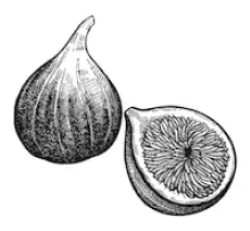
\includegraphics[width=1in,height=1.25in,clip,keepaspectratio]{fig1}}]{Michael Shell}
Use $\backslash${\tt{begin\{IEEEbiography\}}} and then for the 1st argument use $\backslash${\tt{includegraphics}} to declare and link the author photo.
Use the author name as the 3rd argument followed by the biography text.
\end{IEEEbiography}

\vspace{11pt}

\bf{If you will not include a photo:}\vspace{-33pt}
\begin{IEEEbiographynophoto}{John Doe}
Use $\backslash${\tt{begin\{IEEEbiographynophoto\}}} and the author name as the argument followed by the biography text.
\end{IEEEbiographynophoto}




\vfill

\end{document}


